

\section{Fundament der Anwendung}

Das Fundament f\"ur die grafische Oberfl\"ache der Software befindet sich im Webdokument \emph{index.html}.
Es gibt die Struktur der Webanwendung vor.
Zus\"atzlich werden hier auch alle notwendigen Skripte und Stylesheets
im \emph{header} und \emph{body} der \emph{index.html}-Datei eingebunden.
Neben der Struktur befinden sich bereits einige Buttons f\"ur die Navigation im Dokument.
Die Hauptinhalte der Websoftware werden erst zur Laufzeit dynamisch mit JavaScript \"uber das 
DOM-Konzept erzeugt und in das Dokument nachgeladen.
Die Abbildung 5.3 veranschaulicht mit einem Wireframe das Layout der Anwendung.

\begin{figure}[h]
\centering
  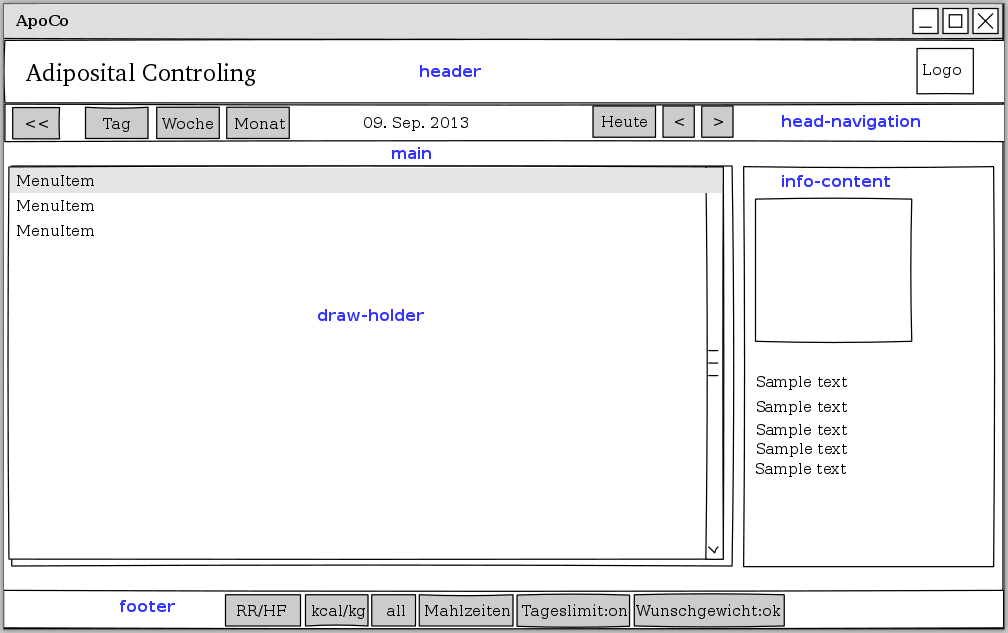
\includegraphics[scale=0.4]{screenshots/kapitel5/wireframe.png}
  \caption{Wireframe f\"ur die Struktur der Webanwendung}
\end{figure}

Im \emph{header}-Bereich befindet sich der Titel der Anwendung (\emph{Adipositas-Controlling}) und ein Logo.
Der Bereich \emph{head-navigation} beinhaltet Buttons f\"ur die Datumsnavigation und einen Button f\"ur die 
R\"uckkehr zur Startseite.
Im \emph{main}-Bereich befinden sich zwei Container.
Der erste wird als \emph{draw-holder} und der zweite als \emph{info-content} bezeichnet.
In beiden Containern werden Informationen zu einem Patienten dargestellt.
Dabei werden diese Informationen im Container \emph{draw-holder} als Graph oder Liste pr\"asentiert.
Im Container \emph{info-content} werden die Informationen in Textform dargestellt.
Unten im Layout der Websoftware befindet sich der Container \emph{footer}.
Hier sind Buttons vorhanden, die zum Filtern der Informationen im Graphen dienen.
Nach dem Start der Software sind zwar bereits alle Buttons im Dokument enthalten, 
werden aber mittels CSS ausgeblendet.
Erst wenn der Benutzer einen Patienten aus einer Liste ausw\"ahlt, 
werden die Inhalte in die Webseite dynamisch eingebaut und 
die n\"otigen Schaltfl\"achen ein und ausgeblendet.
